\documentclass[12pt,a4paper]{ufpr}
% \usepackage[portuges,brazil]{babel}
% \usepackage[portuguese,brazil]{babel}

%instalar aspell-pt

\usepackage[brazil]{babel}
%\usepackage[utf8x]{inputenc} - para corrigir o erro de caractere especial no titulo do cap 1
\usepackage[utf8]{inputenc}
\usepackage{amssymb,amsmath}
\usepackage{epsfig}
\usepackage{multirow}
\usepackage[table,xcdraw]{xcolor}
\usepackage{lmodern}
\usepackage{textcomp} 
\usepackage[T1]{fontenc}
\usepackage{amssymb}
\usepackage{subfigure}
\usepackage{graphicx}
\usepackage{caption}
\usepackage{setspace}
\usepackage{ps-macros}
\usepackage{comment}
\usepackage{url}
\usepackage{listings}
\usepackage{datagidx} %usado para siglas
\usepackage{notoccite}

\newcommand{\specialcell}[2][c]{%
  \begin{tabular}[#1]{@{}c@{}}#2\end{tabular}}

\setcounter{secnumdepth}{3}    % n - numero de niveis de subsubsection numeradas
\setcounter{tocdepth}{3}       % coloca ate o nivel n no sumario

\title{Uma abordagem prática à extração, modelagem e armazenamento de informações de redes sociais}
% \author{Lucas Affonso Xavier de Morais 000 Evelim Carla Ribeiro 000 Alan Peterson Carvalho Silva}
\advisortitle{Orientador} % ou Orientador
\advisorname{Bruno M\"uller Junior.}
\advisorplace{Departamento de Inform\'atica, UFPR}  % departamento, instituicao
\city{Curitiba}
\year{2015}

\banca        % nao insira o nome do orientador, ja eh feito automaticamente
{Prof. ---- }{Departamento de Inform\'tica, UFPR}
{Prof. ---- }{Departamento de Inform\'tica, UFPR}
{}{} % Se houverem outros, preencher
{}{}
\defesa{?? de julho de 2015} % dia em que foi realizada a defesa da dissertação

\newgidx{glossary}{Lista de abreviaturas}
\DTLgidxSetDefaultDB{glossary}

% Dicionariop de siglas
\newterm[description={Sistema de gerenciamento de banco de dados}]{\textbf{SGBD}}

\begin{document}

\makecapaproposta              % cria capa para proposta%
%\makecapadissertacao            % cria capa para dissertacao de mestrado %
%\makerosto                     % cria folha de rosto para versão final da UFPR %
%\maketermo                     % cria folha com o termo de aprovação da dissertação%

%\singlespacing           % espacamento 1 - capa UFPR%
%\onehalfspacing          % espacamento 1/2 %
\doublespacing            % espacamento 2 - UFPR %

\pagestyle{headings}
\pagenumbering{roman}

\chapter*{Agradecimentos}
%Texto de agradecimento
texto de agradecimento          % possiu somente o texto

%\tableofcontents

\listoffigures         
\addcontentsline{toc}{chapter}{\MakeUppercase{Lista de Figuras}}
\newpage

\listoftables        
\addcontentsline{toc}{chapter}{\MakeUppercase{Lista de Tabelas}}
\newpage

\printterms[columns=1,style=align]
%Term definitions

\chapter*{Resumo}
\addcontentsline{toc}{chapter}{\MakeUppercase{Resumo}}
%Texto do resumo.... NAO EDITAR APOCALIPSE PDOE ACONTECER SERIO CUDIADO | EDIT: EU NAO ACREDITO ERA O ACENTO DESGRACADO NAO ESPERAVA PRO ESSA AGORA O TAL DO UNICODE ERA UM MALDITO DUM ACENTO NEM SEI SE ACENTO EH COM C OU COM S MAS ESCREVO BOA TARDE
	
	resumo resumo
	
\textbf{Palavras-chave:} palavras chaves           % somente o texto
\newpage

\chapter*{Abstract}
\addcontentsline{toc}{chapter}{\MakeUppercase{Abstract}}
\textit{abstract}

\textbf{Keywords:} abstract.        % somente o texto
\newpage

\pagenumbering{arabic}

\chapter{Introdução}
\label{Introducao}
%internet
O uso da internet no Brasil vem crescendo a cada ano. Dados oficiais do Banco Mundial apontam que em 2013, 51,6\% da população brasileira tinha acesso à internet, colocando o Brasil na 83a posição no ranking mundial de uso de internet\cite{googlePublicData}.

Uma pesquisa publicada em fevereiro de 2014 pela Pew Research Center\cite{pewPage}, indica que 75\% dos adultos do Brasil acessavam a internet diariamente, sendo que destes, 86\% a utilizavam para acessar redes sociais.
    % Colocar um gráfico aqui (Revisão Bruno)
    
O aumento do número de seus usuários, aumentou também o volume de informações geradas.\cite{domoPage} % affonso: achei meio bosta.

% redes sociais
No Brasil, entre as pessoas que acessam a internet, cerca de 73\% usam redes sociais\cite{BrasilRedesSociais}. No mundo cerca de 1.32 bilhões de pessoas são usuários ativos mensais do Facebook, tornando-o a rede social mais acessada do mundo\cite{investorFacebook}. A segunda \textit{mídia social}\footnote{Websites e aplicações que permitem os usuários criar e compartilhar conteúdo ou participar em redes sociais.\cite{socialMedia}}mais acessada é o Youtube com mais de 1 bilhão de usuários\cite{estatisticasYoutube}.

Esse volume de pessoas acessando as redes sociais e o conteúdo gerado através desses domínios, desperta o interesse de várias áreas para essas ferramentas de interação social.

Uma área que possui vários estudos sobre o uso dessa ferramenta de comunicação é a Ciência da Computação\cite{Benevenuto}. Entre estes, existe o estudo sobre extração de dados em redes sociais, que tem como motivação a quantidade de conteúdo gerada através desses sítios. Como exemplo, somente o Youtube gera cerca de 300 horas de vídeos por minuto \cite{estatisticasYoutube}.

Parte das publicações contidas em redes sociais são públicas. É comum encontrar postagens sobre relacionamentos, oportunidades de emprego, opiniões, entre outros. Este tipo de informação pode ser entendido como uma fonte significativa de informação compartilhada de onde é possível fazer, por exemplo, análises de sentimento deste grupo populacional.

Uma das formas de se fazer a análise é através do uso da estatística. Até o começo do século XXI, uma análise estatística era feita através de pesquisas ou entrevistas feitas por voluntários, o que tornava a maioria dos resultados baseados em pequenas amostras de dados, resultando em estatísticas pouco representativas\cite{Benevenuto}.

Através da extração de dados dessas redes, podemos obter informações sobre qualquer assunto em nível mundial, proporcionando uma base de dados alinhada com a realidade.

\section{Objetivo}

O objetivo é descrever um mecanismo de extração da informação contida em redes sociais e submeter esta informação a ferramentas estatísticas para análise. Para tal foi desenvolvida uma aplicação capaz de (1) extrair informações específicas, (2) armazená-la em um banco de dados e (3) aplicar uma análise estatística sobre estas informações.

No capítulo 2 explicaremos as principais ferramentas e conceitos utilizados como: as APIs das redes sociais estudadas, o framework de desenvolvimento, o sistema gerenciador de banco de dados e uma ferramenta estatística.
No capítulo 3 mostraremos uma visão geral da aplicação e seu funcionamento, e no capítulo 4 detalharemos o processo de pesquisa. E por fim apresentaremos os resultados obtidos no capítulo 5, com o auxílio da ferramenta SentiWordNet\footnote{SentiWordNet é um recurso léxico para mineração de opinião que atribui para cada conjunto de palavras sinônimos três "pontuações de sentimento": positividade, negatividade e objetividade \cite{SentiWordNet}.}.

% \section{Organização do trabalho}

% Este trabalho está dividido em quatro partes. A primeira parte trata os conceitos que foram utilizados para o desenvolvimento do tema, como aplicações web escaláveis, programação orientada a eventos, Javascript e NoSQL. 

% Na segunda parte explicamos mais detalhadamente as tecnologias do MEAN que foram propostas, enfatizando algumas características que contribuem para a escalabilidade.

% A terceira parte aborda como os componentes do MEAN são integrados, além de  mostrar um comparativo de uma aplicação MEAN com o LAMP. O LAMP é outra tecnologia bastante difundida, que utiliza o sistema Linux, o servidor Apache, o banco de dados MySQL e a linguagem de programação PHP\footnote{Podendo haver váriações com outras linguagens de programação como Python e Perl}. Os testes de desempenho também serão apresentados nesta parte.

% A conclusão do trabalho e os possíveis trabalhos futuros são apresentados na quarta e última parte.
\chapter{TECNOLOGIAS}
\label{cha: Conceituacaoo e Ideia Geral}

Nas seções a seguir explicaremos os principais conceitos que utilizaremos para o desenvolvimento do nosso trabalho, as ferramentas utilizadas, fontes de dados exploradas e tecnologias aproveitadas para melhorar o entendimento do tema de nosso trabalho. 

A seção \ref{sec: Redes sociais} descreve as principais redes sociais que podem ser usadas em nossa aplicação, e a seção \ref{sec: API} relata o uso de suas APIs.
A seção \ref{sec: analiseSentimento} contextualiza um dos possíveis usos futuros de nossa aplicação.
Em \ref{sec: Cloud9} é apresentado o ambiente de desenvolvimento em nuvem que utilizamos durante o desenvolvimento da aplicação.
Já a seção \ref{sec: Framework} define o termo Framework, a \ref{sec: MVC} apresenta o padrão de projeto que usaremos, e na seguinte, \ref{sec: Ruby} explica o básico da linguagem de programação que escolhemos para nossa aplicação.
A seção \ref{sec: Rails}, mostra o framework escolhido para o desenvolvimento do trabalho. 
Na seção \ref{sec: BDRelacional} apresentaremos o conceito de banco de dados. % SGBD: colocar no dic. de siglas.
% e, em suas subseções, \ref{subsec: BDRelacional} e \ref{subsec: ActiveRecord} são explicados o conceito de um banco de dados relacional e a biblioteca responsável pelo gerenciamento dos dados, respectivamente.
% e em suas subseções \ref{subsec: FacebookAPI}, \ref{subsec: RedditAPI}, \ref{subsec: YoutubeAPI} e \ref{subsec: TwitterAPI}, serão explicadas as APIs do Facebook, Reddit, Youtube e Twitter, respectivamente.  % mudar esquema das subsecoes

\section{Redes sociais}
\label{sec: Redes sociais}
Rede social é um site dedicado ou um aplicativo que permite que os usuários se comuniquem uns com os outros por meio da publicação de informação, comentários, mensagens, imagens, vídeos ou outros recursos \cite{socialNetworkDefinition}.

Com a popularização da internet, surgiram vários sites que possuem essa estrutura, alguns deles já não existem mais, como o Orkut, já outros recebem muitos acessos ainda hoje como Facebook, Twitter, Youtube, Google+, MySpace, LinkedIn, Reddit, Instagram e Tumblr \cite{wsj}.

Para se ter uma ideia da proporção de pessoas que acessam essas estruturas sociais, considere se o número de usúarios do Facebook fosse a população de um país, ele se tornaria o país mais populoso do mundo \cite{facebookPais}.
Nessa seção apresentaremos uma visão sobre as redes sociais que fazem parte da base do nosso trabalho:  seção \ref{subsec: Facebook} Facebook, seção \ref{subsec: Reddit} Reddit, seção \ref {subsec: Twitter} Twitter, e na seção \ref{subsec: Youtube}  Youtube. Os textos contidos neles possuem conteúdo de caráter opinativo, o que é favorável para aplicações de análise de sentimento.

    \subsection{Facebook}
    \label{subsec: Facebook}
É uma rede social que visa conectar as pessoas aos seus familiares e amigos \cite{FBnewsroom}, permitindo que o usuário crie um perfil, publique textos, fotos, vídeos, envie mensagens e mantenha contato com quem deseja. Foi criada em 2004 por estudantes da Universidade de Harvard e hoje é a maior rede social do mundo, com mais de 1 bilhão de usuários \cite{Facebook101}.

    \subsection{Reddit}
    \label{subsec: Reddit}
É uma comunidade online de mídia social que permite que seus usuários votem e comentem nos conteúdos postados. Podem ser criadas sub-comunidades, chamadas sub-reddits, cujos conteúdos são independentes do Reddit, normalmente com um assunto em comum e moderadas por um grupo de voluntários \cite{WhatIsReddit}. \par
O Reddit é uma fonte de novidades e assuntos populares na internet. Seus usuários produzem o conteúdo e votam em conteúdos postados por outros. Os que recebem grandes quantidades de votos positivos da comunidade, tendem a aparecer no topo da página, sendo assim a página principal mostrará conteúdos novos e relevantes para os leitores \cite{RedditWiki}.
    
    \subsection{Twitter}
    \label{subsec: Twitter}
O Twitter é uma rede social que permite que seus usuários enviem e leiam mensagens curtas de no máximo 140 caracteres chamadas “tweets”.

Atualmente, o Twitter está entre os 10 sites mais acessados do mundo \cite{twitterOverview}, com 288 milhões de usuários ativos por mês e 500 milhões de tweets por dia \cite{aboutTwitter}.

Muitos usuários desse serviço o usam para postar sua opinião sobre outros serviços ou produtos, seja ela uma reclamação ou um elogio, e isso torna essa rede uma importante fonte de dados para nossa aplicação \cite{PAK10.385}.

    \subsection{Youtube}
    \label{subsec: Youtube}
O Youtube foi fundando em maio de 2005 com a finalidade de proporcionar a seus usuários a pesquisa, o entretenimento e o compartilhamento de vídeos em formato digital \cite{SobreYoutube}.

Esse sítio também é considerado uma rede social, pois possui as seguintes características \cite{Benevenuto}:
\begin{enumerate}
    \item Permite construir um perfil publico, ou semipúblico;
    \item Proporciona ao usuário uma lista de outros usuários com os quais ele(a) pode compartilhar informações;
    \item Possibilidade de visualizar e percorrer suas listas de conexões ou as listas criadas por outros usuários.
\end{enumerate} 

O que torna essa rede social relevante para este trabalho é a possibilidade de usuários comentarem em vídeos armazenados por outros usuários da rede, assim expondo sua opinião, seja ela positiva ou negativa, sobre o tema abordado no vídeo.

Os comentários são o principal meio de comunicação entre os usuários do Youtube, e isso os torna uma fonte importante para extração de dados.
Os usuários podem indicar se gostaram de uma publicação específica através do botão \textit{like}, ou se não gostaram através do botão \textit{dislike}. Isto possibilita avaliar quais publicações são mais populares e as menos. Estas características o tornaram um bom candidato para executar a nossa aplicação.

\section{API}
\label{sec: API}

Chamamos de API (Application Programming Interface) um conjunto de comandos, protocolos e funções estabelecidos por um software, com a finalidade de acessar suas funcionalidades sem precisar conhecer seus detalhes de implementação \cite{APIDef}.

Utilizaremos \textbf{APIs web}, que geralmente usam requisições HTTP\footnote{Protocolo usado na transferência de dados pela internet \cite{HTTPDef}.} para enviar mensagens a servidores específicos, que por sua vez retornam uma resposta HTTP geralmente nos formatos XML\footnote{XML é usado para descrever documentos em um formato padrão que pode ser lido por qualquer aplicação compatível com XML \cite{XMLDef}.} ou JSON\footnote{JSON é um formato para trocas de dados estruturados baseados em texto. JSON é comumente usado como uma alternativa ao XML, pois sua forma de representar os dados é mais compacta \cite{JSONDef}.}, com o conteúdo referente à requisição feita.
Toda requisição feita a uma API web precisa de autorização. Para isso a maioria das APIs web utilizam um protocolo chamado OAuth 2.0, que funciona sobre o HTTP e gerencia as autorizações através de uma chave de acesso chamada \textit{access token}.

Na seção acima apresentamos os principais usos das redes sociais Facebook, Reddit, Twitter e Youtube. Como cada uma possui um foco diferente, é natural que cada API aborde da melhor forma seu contexto predominante.

Abaixo iremos explicar as especificidades de cada uma das APIs que usaremos neste trabalho.

% \begin{figure}[ht]
%   \centering
%   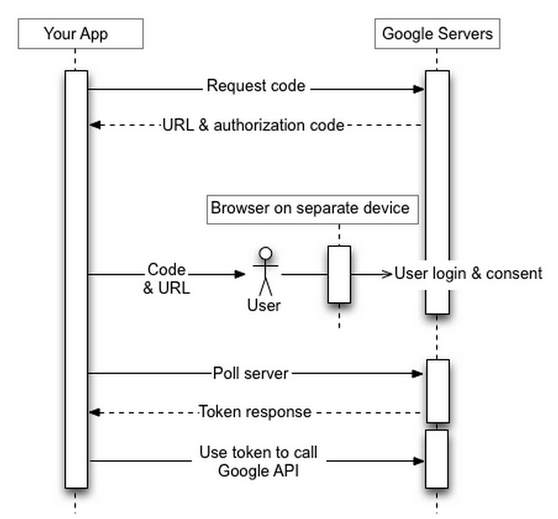
\includegraphics[width=.8\textwidth]{images/accessToken}
 
%   \caption{Procedimento da conta de serviço obtendo o token de acesso \cite{JSONDef}.}
%   \label{fig:accessToken}
% \end{figure}

% Vamos tomar como exemplo o funcionamento de uma requisição à API do Google. As credenciais de uma conta de serviço, que se obtém do Google Developers Console, inclui um endereço de e-mail gerado, que é único, um ID do cliente, e pelo menos um par de chaves: pública e privada. Usa-se o ID do cliente e a chave privada para criar um JWT\footnote{JSON Web Token (JWT) é uma forma compacta de representar reivindicações a serem transferidas entre duas partes. Essas reivindicações em um JWT são codificadas em um objeto no formato JSON e criptografadas ou assinadas digitalmente \cite{APIDef}.} assinado e construir uma solicitação de token de acesso no formato adequado. O seu aplicativo envia a solicitação para o Google OAuth Server 2.0, que retorna um token de acesso. O aplicativo usa o token para acessar uma API do Google. Quando o token expira, repete-se o processo \cite{JSONDef}.

    \subsection{Facebook API}
    \label{subsec: FacebookAPI}
Outra API que possibilitaria uma excelente extração de dados para o nosso sistema é a do Facebook, pois além da pesquisa de publicações públicas, poderíamos também usar as curtidas em fanpages de cada pessoa, para filtrar opiniões de usuários que demonstrem interesse no assunto procurado.

Nós conseguimos utilizar a API do Facebook, entretanto sua atualização para a versão 2.0 e as seguintes conta com uma grande alteração nas permissões que um aplicativo pode utilizar, duas delas impactam diretamente no nosso:
\begin{itemize}
  \item Indisponibilizada a pesquisa de objetos públicos, como as publicações que pretendíamos utilizar \cite{FacebookDevs}.
  \item Indisponibilizado o acesso à lista de amigos de um usuário que não usa seu aplicativo \cite{FacebookDevs}.
\end{itemize}

Estas permissões foram retiradas porque algumas pessoas se sentiam desconfortáveis ao ter suas informações sendo acessadas sem sua permissão direta, como explicado no vídeo oficial do canal Facebook Developers \cite{FbAPIV2Video}.
Como nosso aplicativo depende que as APIs forneçam acesso aos dados públicos dos usuários e o Facebook revogou-os nas versões 2.0 e posteriores da API, tivemos que descartá-lo como fonte de dados.

    \subsection{Reddit API}
    \label{subsec: RedditAPI}
O reddit disponibiliza uma série de informações por sua API, em formato JSON, disponíveis por requisições HTTP simples \cite{RedditAPIWordpress}.
Os recursos\footnote{Um recurso é um conjunto de dados que representa um determinado objeto.} que utilizaremos para construção da nossa aplicação são:
\begin{itemize}
    \item Listing - Uma lista de links.
    \item Comment - Um objeto que representa um comentário em um link.
    \item Client - Um objeto “cliente”, no nosso caso usaremos um usuário e senha em branco, para que criemos um cliente anônimo.
\end{itemize}
Os demais recursos podem ser encontrados no anexo \ref{fig: RecursosReddit}.
Cada recurso permite o uso de um conjunto de operações, por exemplo, um recurso Client, pode executar a operação \textit{search} que irá retornar uma \textit{Listing} (lista de links) que contém os termos passados como parâmetro para a operação \cite{RedditAPISearch}.

Outra operação muito útil para nossa aplicação é a Comments. Executada por um recurso Client, essa operação retorna uma árvore de comentários do link passado por parâmetro, comentários esses que também servirão como textos a serem armazenados pela nossa aplicação.
%[5]
    
    \subsection{Twitter API}
    \label{subsec: TwitterAPI}
A API do Twitter provê acesso à leitura e escrita de dados no Twitter através de requisições HTTP, que podem ser invocadas por códigos escritos em alguma linguagem de programação. Hoje, a versão mais recente da API do Twitter é a 1.1 \cite{TwitterRestApi}.

Algumas possíveis ações são: criar um novo tweet, ler o perfil de um usuário da rede e buscar tweets públicos que possuem um termo em comum \cite{TwitterRestApi}.

Requisições HTTP feitas usando a API do Twitter possuem parâmetros, sendo alguns necessários e outros opcionais. Por exemplo, para buscarmos tweets através de um termo específico devemos especificar o termo em questão como um parâmetro \cite{TwitterSearchApi}.

A URL\footnote{URL, do inglês "Uniform Resource Locator" é o endereço de um site específico da Web ou de um arquivo na Internet \cite{URLDef}.} de uma requisição HTTP a API do twitter versão 1.1 possui o seguinte formato: https://api.twitter.com/1.1/recurso?parametros, substituindo “recurso” e “parâmetros” conforme as necessidades aplicação.

    \subsection{Youtube API}
    \label{subsec: YoutubeAPI}
A API de dados do YouTube (versão 3) permite buscar resultados de pesquisa e recuperar, inserir, atualizar e excluir recursos, como vídeos ou playlists \cite{YouTubeAPI}.

Para criar uma aplicação utilizando a API do Youtube, é necessário criar uma conta no Google para acessar o Console de APIs do Google, solicitar uma chave da API e cadastrar seu aplicativo (caso queira cadastrar um aplicativo veja o apêndice \ref{sec: CadastrandoApp}) \cite{GettingStartedYoutubeAPI}. Com a aplicação cadastrada, temos acesso aos recursos da API. Alguns tipos de recursos da API do Youtube são \cite{GettingStartedYoutubeAPI}:

\begin{itemize}
  \item channel: Contém informações sobre um canal\footnote{ Página principal de uma conta no Youtube.} simples do YouTube.
  \item guideCategory: Identifica uma categoria que o YouTube associa aos canais com base em seu conteúdo ou outros indicadores, como a popularidade.
  \item search result: Contém informações sobre um vídeo, um canal ou uma playlist do YouTube que corresponde aos parâmetros de pesquisa especificados em uma solicitação da API.
\end{itemize}

Outros exemplos de recursos serão encontrados na tabela \ref{fig: RecursosYoutube} nos apêndices \ref{cha: apendices}.

Alguns recursos são compatíveis com operações que executam funções mais específicas a esses recursos. Por exemplo, o recurso search result tem uma operação que recupera uma lista, no qual pode estar vazia ou conter vários recursos \cite{GettingStartedYoutubeAPI}.

Existem operações que precisam de autorização para usar um recurso. Mas existem outras, como a list que não precisam de autorização para serem usadas. 

Nos anexos, pode-se encontrar a tabela \ref{fig: OperacoesCompativeis} que lista as outras operações da API, e a tabela \ref{fig: OperacoesCompativeisComRecursos} que exibe as operações que são compatíveis com cada recurso.

Cada operação tem um custo, que é determinado pela quantidade de memória, CPU e de recursos de rede. Então para garantir que os desenvolvedores usem o serviço de uma forma justa, o Google impõe uma quota, que é um limite de operações que a aplicação pode fazer em um determinado intervalo de tempo \cite{GettingStartedYoutubeAPI}.

Para evitar a transferência, a análise e o armazenamento de dados desnecessários, a API permite a recuperação de recursos parciais. Para isso, esta é compatível com dois parâmetros de solicitação, que permitem identificar as propriedades de recursos que devem ser incluídas nas respostas da API.

\begin{itemize}
	\item O parâmetro part identifica grupos de propriedades que devem ser devolvidas a um recurso. 
	\item O parâmetro fields filtra a resposta da API para devolver apenas propriedades específicas nas partes de recurso solicitadas.
\end{itemize}

\section{Análise de sentimento}
\label{sec: analiseSentimento}
A Análise de sentimento é um campo de estudo que analisa as opiniões, sentimentos, avaliações, atitudes e emoções expressadas por pessoas por meio de textos\cite{ASOpinionMining}.
Desde 2000, vem crescendo para ser uma das áreas de pesquisa mais ativas no processamento de linguagens naturais \cite{ASOpinionMining}. Difundiu-se de ciência da computação para ciências empresariais e ciências sociais, devido a sua importância aos negócios e sociedade como um todo \cite{ASOpinionMining}.

A importância crescente da análise de sentimento coincide com o crescimento da mídia social, tais como comentários, fóruns de discussão, blogs, micro-blogs, Twitter e redes sociais \cite{ASOpinionMining}. Pela primeira vez na história humana, temos agora um enorme volume de dados opinativos gravados em formato digital para análise \cite{ASOpinionMining}.

A análise de sentimento aborda várias áreas de pesquisa. No presente trabalho, utilizaremos a medição de quão negativa ou positiva são as opiniões de um grupo de indivíduos \cite{ASFerreiraEBA}. Os dados de entrada para a análise de sentimento são aqueles tornados públicos em redes sociais.

Utilizando a análise de sentimento, esses dados podem passar de simples textos dentro de um banco de dados, para estatísticas sobre a opinião de um conjunto de pessoas acerca de determinados assuntos.

\section{Cloud9}
\label{sec: Cloud9}
A Cloud9 é um ambiente de desenvolvimento (IDE) que visa melhorar a codificação e atender as necessidades atuais dos desenvolvedores. Um serviço baseado em Computação em nuvens\footnote{A computação em nuvem é um conceito de utilizar a memória, a capacidade de armazenamento, e os recursos de um servidor compartilhando-os por meio da Internet \cite{ComputacaoNuvem}.}, rodando diretamente do navegador, sem necessidade de instalação de nenhum aplicativo adicional, permitindo também executar, depurar, e criar aplicativos de qualquer lugar, a qualquer hora e com outras pessoas simultaneamente \cite{C9ComoUsar}.

\section{Framework}
\label{sec: Framework}
Em geral, um Framework é uma estrutura básica para alguma coisa específica \cite{FrameworkByMerriam}. Portanto, no contexto de desenvolvimento de software, um Framework é uma base para que desenvolvedores de software possam construir programas para uma plataforma específica \cite{FrameworkDef}.

Existem muitos frameworks diferentes para desenvolvimento de aplicações web, cada um com suas utilidades e funcionalidades. Utilizar um framework apropriado no desenvolvimento de uma aplicação pode economizar uma grande quantidade de tempo, além de manter o código organizado e padronizado, o que gera maior facilidade na manutenção do mesmo \cite{FrameworkDocForge}.

\section{Model-view-controller}
\label{sec: MVC}

A arquitetura \textit{Model-View-Controller} (Modelo-Visão-Controlador) tem como objetivo principal fazer uma ponte entre o modelo mental do usuário humano e o modelo digital que existe no computador \cite{Trygve/MVC}.
Sua infraestrutura é dividida em 3 partes \cite{MVC}:

\begin{itemize}
    \item Modelo (model): Contém todo o conteúdo, lógica de processamento e funções, afim de separar os dados.
    \item Visão (view): pode ser qualquer saída de representação dos dados, como uma tabela ou um diagrama, ou seja, como o nome já diz é a visão externa requerida pelo usuário final.
    \item Controlador (controller): faz a mediação entre os acessos ao modelo e à visão e coordena o fluxo de dados entre eles.
\end{itemize}

Inicialmente construída para solucionar problema em geral de usuários que controlam um conjunto de dados grandes e complexos. No entanto o MVC foi adaptado como uma arquitetura para as aplicações Web \cite{WikipediaMVC}.

Foram criados muitos frameworks (seção \ref{sec: Framework}) de aplicação com base nesse modelo, variando em suas interpretações, principalmente no modo que as responsabilidades MVC são divididas entre o cliente e servidor \cite{WikipediaMVC}.

Os frameworks web MVC mais recentes foram adaptados para um modelo cuja visão e a lógica do controlador estão dentro de um servidor \cite{WikipediaMVC}.

Como a complexidade das aplicações sempre visa a programação orientada a objeto, a separação entre dados e a apresentação das aplicações acaba sendo relevante, logo esse padrão atende a esse problema através da separação das tarefas de acesso aos dados e a lógica \cite{WikipediaMVC}.

\section{Ruby}
\label{sec: Ruby}
Ruby é uma linguagem de programação orientada a objeto\footnote{Programação orientada a objetos é uma tentativa de representar os “objetos” que encontramos no mundo real em um software \cite{ObjectOrientedProgramming}.} criada por Yukihiro Matsumoto.

Assim como Perl\footnote{Pearl: Uma linguagem de programação de alto nível e propósito geral usada especialmente para desenvolvimento de aplicações Web \cite{PerlDef}.}, Ruby é apropriada para processamento de textos, pois além de tratar tudo como um objeto, possui blocos e iteradores especiais que facilitam o manuseio de textos \cite{RubyFAQ}.

Nesse trabalho usaremos Ruby aliado ao framework Ruby on Rails, pois essa linguagem apresenta as funcionalidades necessárias para resolver, de forma eficiente, os problemas que encontramos no desenvolvimento dessa aplicação.

    \subsection{Gemas}
    \label{subsec: Gemas}
Assim como a maioria das linguagens de programação, Ruby também possui bibliotecas de funções. A maioria dessas bibliotecas estão na forma de gemas \cite{RubyLibs}. Dentro de uma gema estão os seguintes componentes:
% respondendo o questinamento do bruno, sobre outros formatos de biblitoecas. Acessando a referência:
% "Most of them are released in the form of a gem. [...] Some other libraries are released as archived (.zip or .tar.gz) directories of source code."

\begin{itemize}
    \item Código (Incluindo códigos para testes e outras utilidades)
    \item Documentação
    \item gemspec
\end{itemize}

O arquivo gemspec contém informações importantes sobre a gema como nome, versão e autores \cite{WhatIsGem}.

Para instalar uma gema, usa-se o gerenciador de pacotes RubyGems, que facilita a criação, o compartilhamento e a instalação dessas bibliotecas \cite{RubyLibs}.

\section{Ruby on Rails}
\label{sec: Rails}
Ruby on Rails é um framework de desenvolvimento web de código aberto e que utiliza a linguagem de programação Ruby \cite{RubyOnRails}. Ele contém o que é necessário para desenvolver aplicações web\footnote{Uma aplicação web é um programa cujo processamento de informações é realizado do lado do servidor e o resultado do processamento é enviado, quando permitido, para o cliente que as requisitou via um navegador de internet \cite{TechTerms}.}, com suporte a banco de dados, de acordo com o padrão de projeto de software Model-View-Controller (MVC) \cite{APIRails}.

    \subsection{Motivação}
    \label{subsec: Motivos Rails}
Tendo em vista que as fontes para nosso software são aplicações web, decidimos optar por desenvolver o nosso programa também como uma aplicação web. Utilizaremos o framework Ruby on Rails por já termos estudado-o anteriormente, possuirmos certa afinidade com a linguagem, rapidez de desenvolvimento que ele proporciona e também por existir ótima documentação para o uso das APIs que precisaremos.

Outro ponto que nos fez optar pelo Ruby on Rails foi a agilidade e facilidade que ele oferece para adaptar a modelagem e informações de bancos de dados, que é um de seus pontos fortes como framework de desenvolvimento web \cite{AtlasWeb}.
    
\section{Banco de dados relacional}
\label{sec: BDRelacional}

Um banco de dados relacional é uma coleção de dados organizados em conjuntos de tabelas descritas formalmente, que permite que os dados possam ser acessados, ou manipulados, de maneiras diferentes sem precisar reorganizar as tabelas de banco de dados \cite{RelDatabase}.
Se um banco de dados suporta o modelo relacional, ele organiza seus dados em relações, que por sua vez podem ser vistas como tabelas. Cada coluna de uma tabela representa um atributo da relação, e as linhas representam aos registros \cite{BancoRelacional}.

Um conceito fundamental em um banco de dados relacional é o conceito de atributo chave, que permite identificar e diferenciar um registro de outro. Utilizando atributos chave é possível estabelecer relacionamentos entre duas ou mais tabelas, além de tornar mais rápido o acesso a elementos, usando índices \cite{BancoRelacional}.
Dois dos fatores que contribuem com o sucesso do modelo relacional em bancos de dados é o forte embasamento matemático \cite{FundamentosBD} na definição dos conceitos utilizados e a uniformização da linguagem de manipulação de banco de dados(SQL) \cite{BancoRelacional}.

\subsection{Sistema de gerenciamento de banco de dados}
\label{subsec: SGBD}

Um sistema de gerenciamento de banco de dados (\gls{SGBD}) é um conjunto de programas de software que permite que usuários criem, editem, atualizem, armazenem e recuperem dados em banco de dados de forma mais prática e segura \cite{SGBD}. 

    \subsection{PostgreSQL}
    \label{subsec: PostgreSQL}
	
O PostgreSQL é um \gls{SGBD} de código aberto com mais de 15 anos de desenvolvimento ativo \cite{SobrePostgreSQL}. Considerado o \gls{SGBD} de código aberto mais seguro e avançado \cite{OverviewPostgreSQL}.
Ele, assim como a maioria dos \gls{SGBD}\textbf{s}, segue o padrão de linguagem SQL\footnote{SQL - Structured Query Language é uma linguagem de consulta e manipulação de bancos de dados.} ANSI\footnote{ANSI - American National Standards Institute} e possui extensões próprias para sua linguagem SQL \cite{SQLIntro}.

    \subsection{Active record}
    \label{subsec: ActiveRecord}

Active Record é a gema utilizada pelo framework Ruby on Rails que representa a camada de modelo da aplicação. Esta camada é responsável pelo Mapeamento objeto-relacional\footnote{Mapeamento objeto-relacional - Técnica de desenvolvimento utilizada para reduzir o trabalho necessário de adaptação de um software programado, usando orientação a objeto para utilizar um bancos de dados relacional. As tabelas do banco de dados são representadas na aplicação como classes, e os registros de cada tabela são representados como instâncias das classes correspondentes \cite{ORM}.}, facilitando a criação e o uso dos objetos da aplicação cujos dados precisam de armazenamento persistente\footnote{Armazenamento persistente: Forma de armazenar dados para continuarem a existir mesmo após o término do programa que os criou \cite{BDOO}.} \cite{ActiveRecordBasics}.

Os objetos Active Record não tem seus atributos definidos diretamente, mas sim, inferidos da definição da tabela que representa sua classe. Caso atributos ou tipos desse objeto sejam adicionados, alterados ou removidos, a mudança será realizada também na base de dados, diretamente \cite{ActiveRecordDocs}.
\chapter{IDEIA GERAL}
\label{conceituacaoEIdeiaGeral} %mudar label
Este capítulo tem como foco expôr o processo de desenvolvimento da nossa pesquisa, e o amadurecimento do tema abordado.

\section{Escolha do tema}
\label{sec: escolhaDoTema}
Durante as eleições de 2014, várias pesquisas foram levantadas em diversas redes sociais sobre a opinião das pessoas a respeito dos atuais candidatos. Analisando essas pesquisas, percebemos que muitas delas, apenas ao comparar o número de menções dos candidatos, não expunham a opinião expressa por trás dessas menções.

Percebemos então que pesquisas em áreas diversas apenas levavam em conta a quantidade de menções, e raramente consideravam se a opinião expressa da pessoa que a fez era positiva, negativa, ou neutra sobre o item mencionado.

Essa realidade nos motivou a desenvolver uma aplicação capaz de gerar uma pesquisa, levando em conta o contexto em que a palavra é encontrada. Tal pesquisa com essa característica poderia mostrar que um número alto de menções nas redes sociais não é garantia de aceitação popular.

No decorrer da pesquisa descobrimos o termo Análise de Sentimento(Seção \ref{sec: analiseSentimento}), que se ajustava com a ideia de analisar as opiniões embutidas nos textos coletados das redes sociais.

Pesquisando mais sobre o assunto, percebemos que o nível de complexidade poderia ser suficiente para dois trabalhos de graduação:
\begin{itemize}
    \item O primeiro sendo responsável por armazenar informações coletadas de redes sociais, de forma organizada e eficiente, em um banco de dados;
    \item O segundo, implementar uma ferramenta que realize a análise de sentimento na língua portuguesa, e aplicá-la nos textos armazenados usando o modelo do primeiro trabalho.
\end{itemize}

\section{Visão geral da aplicação}
\label{sec: visaoGeralDaAplicacao}
Escolhemos implementar o modelo de banco de dados nesse trabalho, já que a análise de sentimentos depende de informações previamente armazenadas.
Portanto, nossa aplicação deve:
\begin{enumerate}
    \item Receber um tema de pesquisa como entrada;
    \item Aplicar métodos de busca em diversas redes sociais;
    \item Armazenar os textos coletados em um banco de dados modelado especialmente para a aplicação da análise de sentimento.
\end{enumerate}

\begin{figure}[ht]
  \centering
  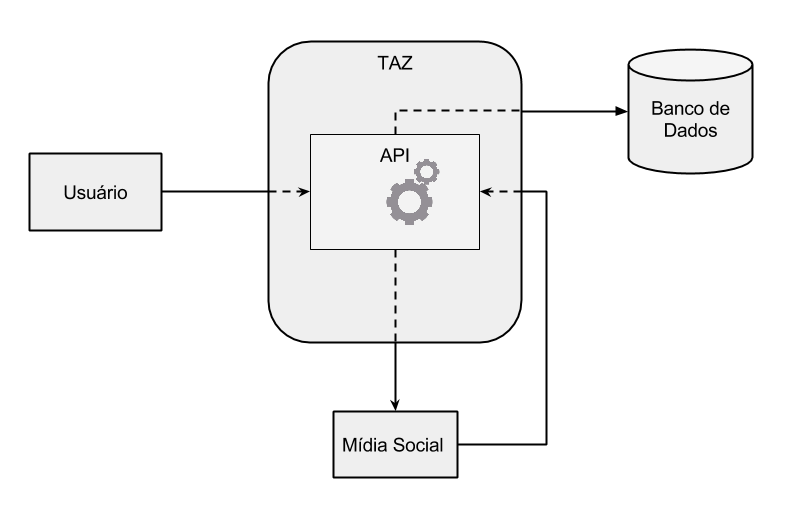
\includegraphics[width=.8\textwidth]{images/esquema}
 
  \caption{Esquema geral da aplicação.}
  \label{fig:esquema}
\end{figure}

Assim, futuros trabalhos nessa área poderão preocupar-se precisamente com a análise em si, sabendo que existem eficientes métodos de pesquisa implementados, e um modelo de banco de dados planejado para este fim, prontos para serem utilizados.
\chapter{Aplicações web com MEAN \textit{Stack}}	 
\label{implementacao}

%\section{Aplicação Math Race  desenvolvido com outras tecnologias}

    No capitulo três foi apresentado cada elemento principal do framework. Neste capítulo será apresentado e analisado, a implementação e funcionamento destes elementos.

Descrição de cada seção comentada.
% Na seção \ref{Comparativo em relação a arquitetura de aplicações LAMP} é apresentado um comparativo entre o MEAN \textit{Stack} e a arquitetura LAMP. A integração das ferramentas do MEAN \textit{Stack} é apresentada na seção \ref{Aplicação Math Race com MEAN Stack}. Na seção \ref{subsec: Testes de desempenho}  são  mostrados os testes realizados em relação ao desempenho.

% A figura \ref{fig:MEAN Stack visto como uma pilha} ilustra a pilha que é formada unindo as tecnologias já explicadas no capítulo anterior. No banco de dados coloca-se o MongoDB, no lado do servidor existe o Node.js e o Express e por último no lado do cliente o AngularJS. A seta de duplo sentido representa que a passagem de dados acontece em ambos os sentidos. O principal motivo para estas tecnologias funcionarem bem em conjunto, é que todas elas têm como base a linguagem Javascript, sendo que esta característica faz parte da proposta do MEAN \textit{Stack} que é o desenvolvimento de aplicações web escaláveis com a utilização de um conjunto de ferramentas em Javascript.
  
    
    % \begin{figure}[htb]
    % \centering
    % \includegraphics[scale=0.5]{images/mean_vs_lamp.png}
    % \caption{Tabela de comparação entre MEAN vs LAMP}
    % \label{fig:tabela mean vs lamp}
    % \end{figure}

Pensamos em deixar a interface com o usuário a mais simples e intuitiva possível.
Para realizar uma extração basta preencher os campos e opções da tela inicial, que consiste em:
\begin{enumerate}
    \item Preencher o campo Keyword\footnote{Palavra chave pela qual será pesquisada. Cada resultado possui ao menos uma vez essa palavra no texto} com a palavra desejada;
    \item Escolher as fontes de extração da informação;
    \item Opcionalmente, adicionar de uma até 3 Tags\footnote{Palavra que simboliza um termo "semelhante parecido sei la, ou relacionado" aos resultados esperados pela busca da Keyword}. Caso o ao menos 1 dos campos Tag seja preenchido, cada resultado irá conter no corpo do texto ao menos 1 "instancia" de "alguma, no minimo dnv" 1 das Tags especificadas;
    \item Clicar no botão Search.
\end{enumerate}

!talvez outra sebseção?
Após preencher o formulário e clicar em Search, o TAZ processa os dados enviados, realiza a pesquisa por 
Keyword AND (Tag1 OR Tag2 OR Tag3)
Caso encontre resultados, realiza a análise de sentimentos nos textos obtidos usando o dicionário/base de dados "nao sei o q eh extamente agr" SentiWordNet.

!talez outra subsec "Apresentando resultados de análise de sentimento"
Com os resultados da análise de cada publicação, calculamos os seguintes dados estatísticos sobre esta amostra:
\begin{itemize}
    \item Média aritmética simples
    \item Média ponderada "BOA TARDe, podemos fazer media ponderada pelo campo de frequencia e explicar o calculo que fizemos numa subsec"
    \item Textos com a \textit{maior} nota positiva
    \item Textos com a \textit{menor} nota positiva
    \item Textos com a nota igual à "mediana"
    \item Textos com a nota igual à "moda"
    \item Desvio padrão dos textos
    https://github.com/jtescher/descriptive-statistics
\end{itemize}

!talvez um capitulo de experimentos
Sobre uma keyword e tags "narrando" os resultados e seus significados

!!sub sec de entrada do experimento

!!sub sec da análise nossa sobre os resultados obervados

!Trabalhos futuros?
O TAS foi desenvolvido sobre um modelo de banco de dados bastante estrito e com a intenção de adaptação fácil a outras tecnologias de "SENTIWORD".
para que possam ser implementados algoritmos de pesquisa em outras fontes basta adicionar o método de pesquisa específico daquela fonte ao controlador de pesquisas (query>contraolle)

!!Para adicionar uma nova fonte
Incluir no banco na tabela Sources do banco de dados o nome da nova fonte.
Adicionar ao controlador "de querys" o algoritmo que realiza a busca na fonte.
(acho que seria legal colocar a assinatura de uma função modelo, tipo Search_<fonte>(query, limit) retornando lista de Posts

!!Para alterar a base de dados de análise de sentimento
Não lembro agr ahhehae mas não é tão difícil acho q eh soh mudar o analyzer






















\section{Aplicação \textit{Math Race} com MEAN \textit{Stack}}
\label{Aplicação Math Race com MEAN Stack}
Nesta seção será apresentada uma aplicação desenvolvida com o MEAN \textit{Stack}. A subseção \ref{subsec: Proposta de desenvolvimento} descreve a proposta de desenvolvimento da aplicação. A subseção \ref{subsec: Utilização e funcionamento da aplicação} mostra como é a utilização e o funcionamento da aplicação. A subseção \ref{subsec: Desenvolvimento da aplicação} aborda como foi desenvolvida a aplicação. 

\subsection{Proposta da aplicação}
\label{subsec: Proposta de desenvolvimento}
 Uma aplicação simples foi desenvolvida, com o intuito de demonstrar diversos aspectos do MEAN \textit{Stack}, como a organização e a integração das ferramentas que compõem o MEAN \textit{Stack}. A aplicação foi baseada na implententação do \textit{Math Race}, desenvolvida por Iván Loire\cite{MathRace}, possuindo apenas o Node.js e o Socket.io como ferramentas em comum.

\subsection{Utilização e funcionamento da aplicação}
\label{subsec: Utilização e funcionamento da aplicação}
 A aplicação é um jogo, cujo objetivo é realizar uma competição em tempo real, para ver qual jogador acerta mais operações de matemáticas aleatórias de adição e subtração, em determinado tempo.

Na figura \ref{fig:Imagem da interface da aplicação} é mostrada a interface da aplicação, que contém a operação aleatória, o campo para entrada de dados, o marcador de tempo (\textit{Time}), o campo de pontuação (\textit{score}) e o Hall da fama (\textit{Hall of fame}).

    \begin{figure}[htb]
    \centering
    \includegraphics[scale=0.3]{images/index_mean_math_race.png}
    \caption{Imagem da interface da aplicação}
    \label{fig:Imagem da interface da aplicação}
    \end{figure}
    
Todos os jogadores possuem o mesmo tempo para responder a mesma operação matemática. A operação matemática muda para todos os jogadores após a resposta correta da operação anterior ter sido preenchida por qualquer jogador.

O jogo funciona através de rodadas, e para cada rodada o usuário tem um tempo limite pré-determinado para acertar o resultado da conta. A cada resultado correto o valor da pontuação do usuário, que começa em zero, é incrementado com mais um ponto. Ao final de uma rodada os usuários que efetuaram alguma pontuação são adicionados no ``Hall da fama'', que é ordenado pelos dez usuários com mais pontos obtidos em uma única rodada, e as pontuações dos usuários são zeradas, para que uma nova rodada se inicie. 

Na figura \ref{fig: Diagrama do funcionamento da aplicação} é demonstrado, através de um diagrama, o funcionameto da aplicação. 

    \begin{figure}[htb]
    \centering
    \includegraphics[scale=0.30]{images/func_mr.png}
    \caption{Diagrama do funcionamento da aplicação}
    \label{fig: Diagrama do funcionamento da aplicação}
    \end{figure}

\subsection{Desenvolvimento da aplicação}
\label{subsec: Desenvolvimento da aplicação}
Nesta subseção será abordado como é o desenvolvimento de uma aplicação baseado no MEAN \textit{Stack}. Partindo de como foi realizada a escolha da estrutura da aplicação, e finalizando com a integração das ferramentas do MEAN \textit{Stack}.
\begin{description}
\item[Estrutura da aplicação] \hfill \\
No início do desenvolvimento da aplicação, verificou-se as possibilidades em relação à estrutura e organização de arquivos que seria utilizada, pois não exite uma abordagem padrão em relação a este assunto.

Nas pesquisas iniciais as primeiras possibilidades que apareceram foram através do MEAN.js e o MEAN.io que são geradores automáticos de estruturas de arquivos para o MEAN \textit{Stack}. Apesar de fornecerem uma estrutura pronta, ao lidar com geradores, é necessário que se programe de uma maneira pré-determinada de acordo com o gerador escolhido, o que torna a aplicação um pouco mais complexa de ser apresentada, e detalhada, e foge do escopo desta monografia.

A opção escolhida para a criação da estrutura de diretórios, foi através de um submódulo do Express.js chamado \textit{express-generator}. A figura \ref{fig: estrutura criada pelo express-generator} mostra como as pastas e os arquivos são organizados neste gerador, ao total são 7 pastas e 9 arquivos. 

    \begin{figure}[htb]
    \centering
    \includegraphics[scale=0.7]{images/estrutura_exp_gen.png}
    \caption{Estrutura criada pelo express-generator \cite{ExpressGen}}
    \label{fig: estrutura criada pelo express-generator}
    \end{figure}

A pasta \textit{public} contém todos os arquivos de imagem, Javascript e CSS que serão enviados para o cliente, como por exemplo os arquivos Javascript do Angular.js, e o arquivo CSS chamado style.css.

Na pasta \textit{views} são definidas as páginas da aplicação, contendo a página do \textit{layout}, do \textit{index}, e uma página de erros. Quando o usuário acessa a aplicação, primeiramente é carregada a página de \textit{layout}, que então carrega a página \textit{index}, e caso algum erro ocorra é enviada uma mensagem de erro.

Para as rotas que definem como serão tratadas as requisições que podem ser realizadas pela aplicação, o \textit{express-generator} cria uma pasta chamada \textit{routes}. Ao receber requisições, o servidor através de funções definidas na pasta \textit{routes}, pode desde renderizar as páginas solicitadas, até encaminhar as requisições para outras rotas, afim de, por exemplo, realizar uma consulta em um banco de dados.

A parte do servidor que o Node.js é responsável, fica no arquivo www da pasta \textit{bin}, e no arquivo app.js na raiz da aplicação.  

Além da estrutura criada pelo \textit{express-generator}, foram criadas mais duas pastas, que são a \textit{models} e a \textit{lib}. Na \textit{models}, ficam os arquivos responsáveis pela conexão e pelos acessos ao MongoDB. A \textit{lib} contém as principais funções da aplicação responsáveis pelo funcionamento do jogo \textit{Math Race}, e da comunicação cliente/servidor, que é feita através do Socket.io, sendo que a sua explicação foi colocada na seção \ref{sec: Socket.io} do apêndice A.

\item[Integração das ferramentas do MEAN \textit{Stack}] \hfill \\
Quando o usuário acessa a aplicação, ocorre uma série de mensagens, entre o lado do cliente e do servidor, afim de informar o servidor que há um novo usuário conectado, e fazer com que o cliente obtenha os dados da partida. 

O diagrama da figura \ref{fig: Diagrama de sequência do acesso da aplicação}, demonstra a sequência de mensagens que ocorrem quando um usuário acessa a aplicação (mensagem 1). 

No lado do servidor, o Node.js envia os arquivos da pasta \textit{public} e o \textit{index} da aplicação (mensagem 2). No lado do cliente, o Angular.js envia uma solicitação de conexão através da função \textit{connect} do Socket.io (mensagem 3), e o Node.js responde com uma mensagem avisando que o usuário está conectado (mensagem 4). Ao receber essa mensagem o Angular.js envia outra mensagem chamada ``\textit{join}'' (mensagem 5), e o Node.js envia os dados referente a operação, a pontuação e o \textit{hall} da fama (mensagem 6, 7 e 8). Por último o Angular.js faz um requisição ao MongoDB para obter o hall da fama atualizado (mensagem 9). 

    \begin{figure}[htb]
    \centering
    \includegraphics[scale=0.7]{images/diagrama_de_seq_acesso.png}
    \caption{Diagrama de sequência do acesso da aplicação}
    \label{fig: Diagrama de sequência do acesso da aplicação}
    \end{figure}
% codigo do join

A cada final de rodada, o Node.js envia uma nova operação, e o Angular.js envia uma mensagem ao Node.js solicitando o \textit{hall} da fama atualizado. Essa mensagem é enviada através de um módulo do Angular.js chamado \textit{ng-resource}, sendo que através deste módulo é possível interagir com o Node.js utilizando o RESTFul\footnote{ ``RESTful é um serviço web que utiliza o paradigma de arquitetura do REST, ou seja, é o termo normalmente usado para se referir a implementação de Web Services que utilizam tal arquitetura.''\cite{RESTWiki}}. 

Caso o usuário tenha efetuado alguma pontuação na rodada, o Angular.js envia uma mensagem ao Node.js, contendo um objeto JSON com o nome e a pontuação efetuada. O Node.js então faz a inserção no MongoDB, se for um novo usuário, ou atualiza a pontuação, se o nome do usuário já estiver cadastrado no MongoDB, e a nova pontuação for maior do que a antiga.

% diagrama demonstrando a aplicação em execução
\end{description}

% \begin{lstlisting}
% 	$scope.sendResult = function(item) {
% 		if (item.value) {
% 		    ...
% 			socket.emit('send-server-result', item);
% 		};
% 	}
% \end{lstlisting}

\section{Testes de desempenho}
\label{subsec: Testes de desempenho}
Nesta seção serão apresentados os testes que foram realizados através de duas aplicações, o \textit{Math Race} e o ``Encurtador de URL''. 

No \textit{Math Race}, foi efetuado um teste simples através do envio de um conjunto de requisições para consultas ao banco de dados, obtendo-se o tempo de duração para o servidor responder cada conjunto de requisições, além da média de requisições por segundo.

A aplicação ``Encurtador de URL'' foi implementada em diversos ambientes, definidos na tabela \ref{fig: Ambientes dos testes}, afim de avaliar o consumo da memória, a utilização da CPU, e a quantidade de requisições realizadas por tempo. 

\subsection{Testes na Aplicação \textit{Math Race}}
% Nesta subseção o objetivo é demonstrar o comportamento da aplicação através de um conjunto de testes de envio de requisições e consultas ao banco de dados. 
Os testes foram realizados aumentando gradativamente a quantidade de requisições e requisições concorrentes, afim de verificar a latência de resposta do servidor. A cada requisição é realizada uma consulta no banco de dados para obtenção da lista dos dez primeiros usuários e suas pontuações no \textit{hall} da fama.

Na figura \ref{fig: Lista de objetos retornada pelo MongoDB}, podemos observar parte da lista de objetos retornada pela consulta ao banco de dados, que cada cliente realiza ao acessar a aplicação durante os testes.

    \begin{figure}[htb]
    \centering
    \includegraphics[scale=0.7]{images/objs_hof_bd.png}
    \caption{Lista de objetos retornada pelo MongoDB}
    \label{fig: Lista de objetos retornada pelo MongoDB}
    \end{figure}
% \begin{lstlisting}
% \end{lstlisting}

A máquina utilizada nos testes tem como configurações um Core i7 de 3.6GHZ, e 8GB de memória RAM, utilizando o Fedora 20 de 64 \textit{bits} como sistema operacional.


Na tabela \ref{fig: Carga na quantidade requisições} são mostrados os resultados dos testes realizados na aplicação, através de uma ferramenta específica para teste de carga (\textit{Load test}) conhecida como \textit{weighttp}\footnote{http://redmine.lighttpd.net/projects/weighttp/wiki}. No \textit{weighttp} é possível definir parâmetros como a quantidade de requisições que serão enviadas ao servidor e o número de requisições concorrentes que ocorrerão durante o teste.

Para estes testes foram imaginados dois cenários diferentes, sendo determinada uma quantidade de requisições concorrentes fixa (100 e 1000) em cada cenário. Para cada cenário variou-se a quantidade de requisições de 1.000 até 100.000, obtendo-se o tempo demorado pelo servidor para atender todas estas requisições e a taxa de requisições por segundo. 


\begin{table}[ht]
\centering
\begin{tabular}{|c|c|c|c|}
\hline
\rowcolor[HTML]{CFCFCF} 
\# requisições concorrentes & \# requisições & tempo(seg) & req/seg      \\ \hline
\rowcolor[HTML]{EFEFEF} 
\cellcolor[HTML]{EFEFEF} & 1000 & 0,69 & 1458  \\ \cline{2-4}
\rowcolor[HTML]{EFEFEF} 
\cellcolor[HTML]{EFEFEF} & 2000 & 1,357 & 1472  \\ \cline{2-4}
\rowcolor[HTML]{EFEFEF} 
\cellcolor[HTML]{EFEFEF} & 5000           & 3,437      & 1454  \\ \cline{2-4} 
\rowcolor[HTML]{EFEFEF} 
\cellcolor[HTML]{EFEFEF} & 10000          & 7,690      & 1414  \\ \cline{2-4} 
\rowcolor[HTML]{EFEFEF} 
\cellcolor[HTML]{EFEFEF} & 30000          & 20,928     & 1433  \\ \cline{2-4} 
\rowcolor[HTML]{EFEFEF} 
\cellcolor[HTML]{EFEFEF} & 50000          & 34,986     & 1429  \\ \cline{2-4} 
\rowcolor[HTML]{EFEFEF} 
\cellcolor[HTML]{EFEFEF} & 70000          & 47,102     & 1486  \\ \cline{2-4} 
\rowcolor[HTML]{EFEFEF}
\multirow{-8}{*}{\cellcolor[HTML]{EFEFEF}100} & 100000 & 67,967     & 1471  \\ \hline
    & 1000           & 3,250      & 330   \\ \cline{2-4} 
    & 2000           & 3,350      & 658   \\ \cline{2-4} 
    & 5000           & 3,691      & 1354  \\ \cline{2-4} 
    & 10000          & 7,503      & 1332  \\ \cline{2-4} 
    & 30000          & 21,963     & 1365  \\ \cline{2-4} 
    & 50000          & 37,327     & 1339  \\ \cline{2-4} 
    & 70000          & 52,157     & 1342  \\ \cline{2-4} 
\multirow{-8}{*}{1000}   & 100000         & 74,914     & 1334  \\ \hline    
\end{tabular}
\caption{Carga na quantidade requisições}
\label{fig: Carga na quantidade requisições}
\end{table}

Pode-se notar através da tabela \ref{fig: Carga na quantidade requisições}, que à medida que carga de requisições aumenta, o tempo  total para o servidor responder estas requisições cresce consideravelmente, independentemente do número de requisições concorrentes, mas mantém, em média, a mesma taxa de requisições por segundo. No gráfico da figura \ref{fig: Gráfico de requisições por tempo}, pode-se visualizar de maneira mais clara o comportamento da aplicação, durante a carga de requisições.  
% \newpage
    \begin{figure}[htb]
    \centering
    \includegraphics[scale=0.7]{images/reqxtempo.png}
    \caption{Gráfico de requisições por tempo}
    \label{fig: Gráfico de requisições por tempo}
    \end{figure}

\newpage

\subsection{Análise de testes de desempenho do Node.js e do MongoDB com outros ambientes}
Os principais componentes responsáveis pela a escalabilidade no MEAN \textit{Stack} são o MongoDB, através do \textit{autosharding}, e do mapeamento dos dados em memória, e o NodeJS, através do \textit{Event Loop}, e da \textit{Thread Pool}, como mencionado no capítulo \ref{tecnologias}.
    
Existem diversas referências que comparam o desempenho destes dois componentes juntos com outros ambientes, variando desde a linguagem de programação até a base de dados utilizada.

A referência que esta monografia irá utilizar como base é a do artigo de Ricardo Schroeder e Fernando dos Santos,  intitulado ``Arquitetura e testes de serviços web de alto desempenho com Node.js e Mongodb'' \cite{NodejsEMongodb} que implementou um ``Encurtador de URL'' como aplicação.

A aplicação do ``Encurtador de URL'' serve para mapear uma \textit{hash}, de 6 caracteres, para uma URL. Cada \textit{hash} é gerada de maneira única, e aleatória, e foram alocados um milhão de URL's para os testes.

A cada acesso é feita a verificação se a \textit{hash} utilizada é válida.  Primeiro é verificado se a \textit{hash} tem 6 caracteres e depois se ela existe no banco de dados, caso alguma destas verificações falhe é retornado somente um código de  resposta de erro 404. 

Para os testes, a aplicação definida foi implementada em 6 ambientes, que foram descritos na tabela \ref{fig: Ambientes dos testes}. Cada aplicação de um ambiente efetua a mesma requisição e será testada utilizando uma base de amostras contendo duas mil \textit{hashs}. A duração foi estipulada em 60 segundos, sendo que nos  5 segundos iniciais, foram criados quarenta usuários que irão se conectar de maneira incremental, permanecendo ativos durantes os próximos quarenta e cinco segundos e reduzindo durante os dez segundos finais. 

\begin{table}[htb]
\centering
\begin{tabular}{|c|c|c|}
\cline{1-3}
\rowcolor[HTML]{CFCFCF}
Servidor & Linguagem de Programação & Banco de Dados \\ \cline{1-3}
Node.JS  & Javascript               & MongoDB        \\ \cline{1-3}
Node.Js  & Javascript               & PostgresSQL    \\ \cline{1-3}
Netty    & Java                     & MongoDB        \\ \cline{1-3}
Netty    & Java                     & PostgresSQL    \\ \cline{1-3}
Apache   & PHP                      & MongoDB        \\ \cline{1-3}
Apache   & PHP                      & PostgresSQL    \\ \cline{1-3}
\end{tabular}
\caption{Ambientes dos testes \cite{NodejsEMongodb}}
\label{fig: Ambientes dos testes}
\end{table}

Os testes realizados na aplicação foram executados em um ambiente virtualizado contendo as seguintes características: Sistema Operacional CentOS 6.2 x86, 1Gb de memória RAM, 2 núcleos de 2,4Ghz Intel Core I5. A aplicação utilizada para os testes foi o JMeter, que é um software que serve para realizar testes de desempenho, carga e stress, desenvolvido pela Apache\footnote{http://jmeter.apache.org/} . Os resultados são mostrados nas tabelas \ref{fig:graf_memoria}, \ref{fig:graf_cpu} e \ref{fig:graf_tempo}.
\clearpage
\begin{description}
\item[Consumo de Memória RAM] \hfill \\
A memória RAM é um dos princípais pontos de análise em um servidor web, pois está ligada diretamente ao número de requisições que o servidor é capaz de atender em determinado tempo.\cite{NodejsEMongodb}
O resultado do teste demonstrou o uso de memória constante e estabilidade por parte de cada plataforma. Os piores resultados ficaram com os ambientes que utilizam o servidor Apache e a linguagem PHP, enquanto o ambiente que usa Node.js e o MongoDB foi o segundo melhor no índice de consumo de memória.

\begin{figure}[htb!]
\centering
\includegraphics[scale=0.5]{images/graf_memoria.png}
\caption{Consumo de memória RAM durante a execução dos testes \cite{NodejsEMongodb}}
\label{fig:graf_memoria}
\end{figure}

\clearpage
 
\item[Utilização de CPU] \hfill \\
Analisar a utilização de CPU é um fator relevante para que se tenha uma noção da carga gerada pelas requisições efetuadas pelos clientes. Quanto mais próximo de 100\% estiver o uso da CPU, maiores serão as chances do servidor não conseguir atender as requisições recebidas. 

No gráfico da figura \ref{fig:graf_cpu} nota-se um melhor desempenho do Node.js junto ao MongoDB em relação aos outros ambientes, ficando com 40\% de uma média de uso, enquanto em outros ambientes como o que utilizou Java/Netty/PostgreSQL este consumo passou para aproximadamente 90\%.

\begin{figure}[htb]
\centering
\includegraphics[scale=0.5]{images/graf_cpu.png}
\caption{Consumo de CPU (\%) durante a execução do teste. \cite{NodejsEMongodb}}
\label{fig:graf_cpu}
\end{figure}

% \newpag
\clearpage
\item[Quantidade de requisições por tempo] \hfill \\
O teste de requisições por tempo basicamente indica o quanto de usuários (requisições) o servidor é capaz de absorver.\cite{NodejsEMongodb}

Na figura \ref{fig:graf_tempo} é possível observar que os dois ambientes que mais responderam requisições, que no caso foram o Node.JS/MongoDB e o Netty/MongoDB, utilizaram o mesmo banco de dados. Mas o crédito desse resultado positivo, também se deve aos servidores de alto desempenho, que possuem como característica atender o maior numero de requisições simultâneas. Outro ponto que chama atenção, é como os ambientes com MongoDB se destacaram sobre os ambientes com PostgresSQL.

% \clearpage
\begin{figure}[htb]
% \centering
\includegraphics[scale=0.5]{images/graf_req_tempo.png}
\caption{Requisições por tempo. \cite{NodejsEMongodb}}
\label{fig:graf_tempo}
\end{figure}

\end{description}


Após ser realizada uma análise dos testes, tanto no \textit{Math Race} quanto no ``Encurtador de URL'', concluímos que realmente a utilização do Node.js junto ao MongoDB, proporciona um ganho de desempenho considerável, em relação as tecnologias comparadas. Este ganho se deve ao fato das particularidades que cada tecnologia adota, para lidar com escalabilidade, no caso o Node.js com o \textit{Event Loop} e o MongoDb com o \textit{Autosharding}.
%de maneira pura, ou seja, sem que haja alteração para obtenção de resultados  



% PROPOSTA DE DESENVOLVIMENTO

% DIAGRAMA DE CASOS DE USO
%  Especificações dos cs

% DESENVOLVIMENTO DA APLICAÇÃO

% UTILIZAÇÃO DA APLICAÇÃO

%  TESTES DE DESEMPENHO
%   weigthttp
%   objetivo do teste, como foram realizados, hardware utilizado
%      analise dos resultados obtidos

%   figura

% analise dos teste


%\chapter{Testes e resultados obtidos}
\label{cha: TestesEResultados}
!talvez um capitulo de experimentos
Sobre uma keyword e tags "narrando" os resultados e seus significados

!!sub sec de entrada do experimento

!!sub sec de resultados obtidos 

!!sub sec de interpretação desses resultados



!!!!!!Talvez na conclusão???

!Trabalhos futuros?
O TAZ foi desenvolvido sobre um modelo de banco de dados bastante estrito e com a intenção de adaptação fácil a outras tecnologias de análise de sentimentos.
para que possam ser implementados algoritmos de pesquisa em outras fontes basta adicionar o método de pesquisa específico daquela fonte ao controlador de pesquisas (query>contraolle)

!!Para adicionar uma nova fonte
Incluir no banco na tabela Sources do banco de dados o nome da nova fonte.
Adicionar ao controlador "de querys" o algoritmo que realiza a busca na fonte.
(acho que seria legal colocar a assinatura de uma função modelo, tipo Search_<fonte>(query, limit) retornando lista de Posts

!!Para alterar a base de dados de análise de sentimento
Não lembro agr ahhehae mas não é tão difícil acho q eh soh mudar o analyzer
%\chapter{Conclusão}
\label{conclusao}

Esta monografia apresentou os conceitos de redes sociais e suas respectivas APIs, além de um breve introdução sobre análise de sentimento. Juntamente com o desenvolvimento de uma aplicação em ruby on rails, que tem como objetivo extrair dados de redes sociais inserindo-as em um banco de dados para análise posterior.
  
  
  
  
  

   
\section{Trabalhos Futuros}
 Para trabalhos futuros, seria interessante implementar uma ferramenta que realize a análise de sentimento na língua portuguesa, e aplicá-la nos textos armazenados usando o modelo deste trabalho.

\chapter{Apêndices}
\label{cha: apendices}

\section{Recursos e tipos de recursos da API do Youtube}
\label{sec: RecursosYoutube}

\begin{table}[ht]
\begin{tabular}{|p{3cm}|p{12cm}|}
\hline
\rowcolor[HTML]{CFCFCF} 
Tipo de recurso	&	Descrição	 \\ \hline
activity	    &	Contém informações sobre uma ação que determinado usuário executou no site do YouTube. Ações do usuário que são informadas em feeds de atividades incluem a classificação de um vídeo, o compartilhamento de um vídeo, a marcação de um vídeo como favorito, a publicação de um boletim do canal etc.	\\ \hline
channel	        &	Contém informações sobre um canal simples do YouTube.	\\ \hline
channelBanner	&	Identifica o URL que será usado para definir uma imagem recém-enviada como imagem do banner de um canal.	\\ \hline
guideCategory	&	Identifica uma categoria que o YouTube associa aos canais com base em seu conteúdo ou outros indicadores, como a popularidade. As categorias de guia servem para organizar canais de modo que os usuários do YouTube possam encontrar com mais facilidade o conteúdo que procuram. Embora os canais possam ser associados a uma ou mais categorias de guia, não é certeza que eles estejam em uma delas.	\\ \hline
playlist	    &	Representa uma playlist simples do YouTube. Uma playlist é um conjunto de vídeos que podem ser visualizados em sequência e compartilhados com outros usuários.	\\ \hline
playlistItem	&	Identifica um recurso, como um vídeo, que faz parte de uma playlist. O recurso playlistItem também contém detalhes que explicam como o recurso incluso é usado na playlist.	\\ \hline
search result	&	Contém informações sobre um vídeo, um canal ou uma playlist do YouTube que corresponde aos parâmetros de pesquisa especificados em uma solicitação da API. Embora indique um recurso exclusivamente identificável (como um vídeo), um resultado de pesquisa não tem seus próprios dados persistentes.	\\ \hline
subscription	&	Contém informações sobre a inscrição de um usuário do YouTube. Uma assinatura notifica o usuário quando novos vídeos são adicionados a um canal ou quando outro usuário executa uma das várias ações no YouTube, como o upload ou a classificação de um vídeo ou comentários sobre um vídeo.	\\ \hline
thumbnail	    &	Identifica imagens em miniatura associadas a um recurso.	\\ \hline
video	        &	Representa um vídeo simples do YouTube.	\\ \hline
videoCategory	&	Identifica uma categoria que foi ou pode ser associada a vídeos enviados.	\\ \hline
\end{tabular}
\caption[Recursos e tipos de recursos]{Recursos e tipos de recursos\cite{GettingStartedYoutubeAPI}.}
\label{fig: RecursosYoutube}
\end{table}

\section{Operações compatíveis}
\label{sec: OperacoesCompativeis}

\begin{table}[ht]
\begin{tabular}{|p{3cm}|p{12cm}|}
\hline
\rowcolor[HTML]{CFCFCF} 
Operação  &	Descrição	\\ \hline
list	  &	Recupera (GET) uma lista vazia ou com recursos.	\\ \hline
insert	  &	Cria (POST) um novo recurso.	\\ \hline
update	  &	Modifica (PUT) um recurso existente para propagar os dados em sua solicitação.	\\ \hline
delete	  &	Remove (DELETE) um recurso específico.	\\ \hline
\end{tabular}
\caption[Operações compatíveis]{Operações compatíveis\cite{GettingStartedYoutubeAPI}.}
\label{fig: OperacoesCompativeis}
\end{table}

\section{Relação de compatibilidade de recursos e operações}
\label{sec: OperacoesCompativeisComRecursos}

\begin{table}[ht]
\begin{tabular}{|p{6cm}|p{2cm}|p{2cm}|p{2cm}|p{2cm}|}
\hline
\rowcolor[HTML]{CFCFCF} 
Tipo de recurso	&\multicolumn{4}{|c|}{Operações suportadas}  \\ \hline
\ &	list	&	insert	&	update	&	delete	\\ \hline
activity	    &	sim		&	sim		&	não		&	não		\\ \hline
channel	        &	sim		&	não		&	não		&	não		\\ \hline
channelBanner	&	não		&	sim		&	não		&	não		\\ \hline
guideCategory	&	sim		&	não		&	não		&	não		\\ \hline
playlist	    &	sim		&	sim		&	sim		&	sim		\\ \hline
playlistItem	&	sim		&	sim		&	sim		&	sim		\\ \hline
search result	&	sim		&	não		&	não		&	não		\\ \hline
subscription	&	sim		&	não		&	não		&	não		\\ \hline
thumbnail	    &	não		&	não		&	não		&	não		\\ \hline
video	        &	sim		&	sim		&	sim		&	sim		\\ \hline
videoCategory	&	sim		&	não		&	não		&	não		\\ \hline
\end{tabular}
\caption[Operações compatíveis com recursos]{Operações compatíveis com recursos\cite{GettingStartedYoutubeAPI}.}
\label{fig: OperacoesCompativeisComRecursos}
\end{table}

\section{Cadastrando um aplicativo}
\label{sec: CadastrandoApp}

Para cadastrar um aplicativo siga o seguintes passos:

\begin{enumerate}
    \item Vá até a página https://console.developers.google.com/project;
    \item Selecione um projeto;
    \item Selecione APIs e autorização. Na lista de APIs, certifique-se que o estado é ON para a YouTube Data API v3.
    \item Selecione Credenciais.
    \item A API é compatível com dois tipos de credenciais. Crie as credenciais apropriadas para seu projeto:
    \begin{itemize}
    	\item OAuth 2.0: seu aplicativo precisa enviar um token do OAuth 2.0 com todas as solicitações que acessam dados privados do usuário. Seu aplicativo envia um ID do cliente e possivelmente uma chave secreta do cliente para conseguir um token. É possível gerar credenciais do OAuth 2.0 para aplicativos na Web, contas de serviço ou aplicativos instalados.
    	\item Chaves de API: Uma solicitação que não fornece um token do OAuth 2.0 precisa enviar uma chave de API. A chave identifica seu projeto e fornece acesso à API, à cota e aos relatórios.
    \end{itemize}
    obs: Se o tipo de chave necessária ainda não existe, crie uma chave de API selecionando Criar nova chave e, então, escolha o tipo apropriado de chave. Em seguida, insira os dados adicionais obrigatórios para esse tipo de chave.
\end{enumerate} 

Em nossa aplicação utilizamos utilizaremos a credencial OAuth 2.0 através de uma conta de serviço, pois queremos as informações públicas dessa rede social.

\begin{table}[ht]
\centering
\begin{tabular}{|p{2cm}|p{3cm}|}
\hline
\rowcolor[HTML]{CFCFCF} 
Prefixo	&	Tipo de link	\\ \hline
t1\_	    &	Comment	        \\ \hline
t2\_	    &	Account	        \\ \hline
t3\_	    &	Link	        \\ \hline
t4\_	    &	Message	        \\ \hline
t5\_	    &	Subreddit	    \\ \hline
t6\_	    &	Award         	\\ \hline
t8\_	    &	PromoCampaign	\\ \hline
\end{tabular}
\caption[API do Reddit - Tipos de recursos e seus prefixos]{API do Reddit - Tipos de recursos e seus prefixos \cite{RedditAPI}.}
\label{fig: RecursosReddit}
\end{table}
      % se houver anexo

\bibliographystyle{brazil} %ordena a bibliografia por ordem alfabética de titulo ou autor...
\bibliography{bibliografia}
%utilize macros (3 primeiras letras do mes em ingles, minusculas) no seu
%.bib para atribuir o nome do mes em portugues nas referencia,
%se o style for brazil, outros estilos tambem aceitam estas macros
%Ex:
%
%@InProceedings{teste,
%  author =       {Luciano}
%  year =         {2013}
%  month =        {}#sep;
%}

\addcontentsline{toc}{chapter}{\MakeUppercase{Bibliografia}}

%\singlespacing
%\makecapadissertacao

\end{document}
